% !TeX root = ../libro.tex
% !TeX encoding = utf8
\chapter{Existencia y unicidad de solución de la ecuación lineal integral de Volterra de segunda clase}
\section{Teorema de la serie geométrica y sus variantes}
El siguiente resultado se usa muy a menudo en análisis numérico y matemática aplicada. También es la forma que tenemos para analizar si tienen solución los problemas que están $"$cerca$"$ a otros problemas que sabemos que tienen solución única.
\begin{teorema}
	(Teorema de la serie geométrica) Sea X un espacio de Banach, $L \in \mathcal{L}(X)$. Suponemos
	\begin{equation}
		\lVert L \rVert \leq 1.
	\end{equation}
	Entonces $I - L$ es una biyección en X, su inversa es un operador lineal continuo,
	\begin{equation}
		(I-L)^{-1} = \sum_{n=0}^{\infty}L^n,
	\end{equation}
	y
	\begin{equation}\label{eq:teo1}
		\lVert (I-L)^{-1} \rVert \leqslant \dfrac{1}{1 - \lVert L \rVert}.
	\end{equation}
\end{teorema}
\begin{proof}
	Definimos una sucesión en $\mathcal{L}(X): M_n = \sum_{i=0}^{n}L^i, n \geqslant 0$. Para $p \geqslant 1$, 
	\begin{equation}
		\lVert M_{n+p} - M_n \rVert = \lVert \sum_{i=n+1}^{n+p}L^i \rVert \leqslant \sum_{i=n+1}^{n+p} \lVert L^i \rVert \leqslant \sum_{i=n+1}^{n+p} \lVert L \rVert^i.
	\end{equation}
	Usando que $\lVert L \rVert \leq 1$, tenemos
	\begin{equation}
		 \lVert M_{n+p} - M_n \rVert \leqslant \dfrac{\lVert L \rVert^{n+1}}{1 - \lVert L \rVert}.
	\end{equation}
	Por tanto,
	\begin{equation}
		\sup_{p \geqslant 1} \lVert M_{n+p} - M_n \rVert \rightarrow 0, \qquad n \rightarrow \infty,
	\end{equation}
	y \{$M_n$\} es una sucesión de Cauchy en $\mathcal{L}(X)$. Como $\mathcal{L}(X)$ es completo, hay un $M \in \mathcal{L}(X)$ tal que
	\begin{equation}
		\lVert M_{n} - M \rVert \rightarrow 0, \qquad n \rightarrow \infty.
	\end{equation}
	Usando la definición de $M_n$ y una simple manipulación algebraica,
	\begin{equation}
		(I-L)M_n = M_n(I-L) = I - L^{n+1}.
	\end{equation}
	Si $n \rightarrow \infty$ obtenemos
	\begin{equation}
		(I-L)M = M(I-L) = I.
	\end{equation}
	Esta relación implica que $(I-L)$ es una biyección, y
	\begin{equation}
		M = (I-L)^{-1} = \lim_{n \rightarrow \infty}\sum_{i=0}^{n}L^i = \sum_{n=0}^{\infty}L^n.
	\end{equation}
	Para probar la desigualdad~\eqref{eq:teo1}, observemos que
	\begin{equation}
		\lVert M_{n} \rVert \leqslant \sum_{i=0}^{n}\lVert L \rVert^i \leqslant \dfrac{1}{1 - \lVert L \rVert}.
	\end{equation}
	Tomando el límite en $n \rightarrow \infty$, obtenemos~\eqref{eq:teo1}.
\end{proof}
\begin{observacion}
	El teorema dice que bajo las hipótesis que hemos marcado, para cualquier $f \in X$, la ecuación
	\begin{equation}\label{eq:teo2}
		(I-L)u = f
	\end{equation}
	tiene solución única $u = (I-L)^{-1}f \in X$. Además, la solución depende continuamente de la parte derecha $f$: Siendo $(I-L)u_1 = f_1$ y $(I-L)u_2 = f_2$, de esto se sigue que
	\begin{equation}
		u_1 - u_2 = (I-L)^{-1}(f_1 - f_2),
	\end{equation}
	y por tanto,
	\begin{equation}
		\lVert u_1 - u_2 \rVert \leqslant c \lVert f_1 - f_2 \rVert
	\end{equation}
	con $c = 1/(1 - \lVert L \rVert)$.
\end{observacion}
\begin{observacion}
	Este teorema también nos da una forma de aproximar la solución de la ecuación~\eqref{eq:teo2}. Bajo las hipótesis del teorema, tenemos
	\begin{equation}
		u = \lim_{n \rightarrow \infty}u_n
	\end{equation}
	donde
	\begin{equation}
		u_n = \sum_{j=0}^{n}L^jf.
	\end{equation}
\end{observacion}
Veamos a continuación un ejemplo en el que, gracias al teorema de la serie geométrica, veremos que una ecuación lineal integral tiene solución única.
\begin{ejemplo}\label{ej:1}
	Sea la siguiente ecuación:
	\begin{equation}
		\lambda u(x) - \int_{a}^{b}k(x,t)u(t)dy = f(x), \qquad a \leqslant x \leqslant b
	\end{equation}
	con $\lambda \neq 0$, $k(x,y)$ continua para $x,y \in [a,b]$, y $f \in \mathcal{C}[a,b]$. Sea $X = \mathcal{C}[a,b]$ con la norma $\lVert \cdot \rVert_\infty$. Simbólicamente, escribimos la ecuación como
	\begin{equation}
		(\lambda I-K)u = f,
	\end{equation}
	donde $K$ es un operador integral lineal gerenado por el núcleo $k(\cdot , \cdot )$. Nosotros también lo escribiremos a menudo como $(\lambda - K)u = f$, para aclarar la notación.
	
	Escribimos la ecuación de esta manera puesto que así se puede convertir en la forma que necesitamos para aplicar el teorema de la serie geométrica:
	\begin{equation}
		(I-L)u = \dfrac{1}{\lambda}f, \qquad L = \dfrac{1}{\lambda}K.
	\end{equation}
	Aplicando el teorema de la serie geométrica, afirmamos que si
	\begin{equation}
		\lVert L \rVert = \dfrac{1}{|\lambda |}\lVert K \rVert \leq 1,
	\end{equation}
	entonces $(I-L)^{-1}$ existe y
	\begin{equation}
		\lVert(I-L)^{-1}\rVert \leqslant \dfrac{1}{1 - \lVert L \rVert}.
	\end{equation}
	Equivalentemente, si
	\begin{equation}
		\lVert K \rVert = \max_{a\leqslant x\leqslant b}\int_{a}^{b}|K(x,t)|dt \leq |\lambda|,
	\end{equation}
	entonces $(\lambda I - K)^{-1}$ existe y 
	\begin{equation}
		\lVert (\lambda I - K)^{-1}\rVert \leqslant \dfrac{1}{|\lambda| - \lVert K \rVert }.
	\end{equation}
	Luego, para cualquier $f \in \mathcal{C}[a,b]$, la ecuación integral tiene solución única $u \in \mathcal{C}[a,b]$ y 
	\begin{equation}
		\lVert u \rVert_\infty \leqslant \lVert (\lambda I - K)^{-1} \rVert \lVert f \rVert_\infty \leqslant \dfrac{\lVert f \rVert_\infty}{|\lambda| - \lVert K \rVert }.
	\end{equation}
\end{ejemplo}
\begin{observacion}
	Gracias a la demostración del teorema podemos ver que para un operador lineal $L \in \mathcal{L}(X)$ sobre un espacio de Banach $V$, si $\lVert L \rVert \leq 1$, entonces la serie $\sum_{n=0}^{\infty}L^n$ converge en $\mathcal{L}(X)$ y el valor de la serie es el operador $(I-L)^{-1}$.
\end{observacion}
\subsection{Generalización del teorema}
Para motivar la generalización del teorema, vamos a considerar la ecuación integral de Volterra de segunda clase
\begin{equation}
	u(x) - \int_{0}^{x} K(x,t)u(t)dt = f(x), \qquad x \in [0,B],
\end{equation}
donde $B \geq 0$ y suponemos que el núcleo $K(x,t)$ es continuo para $0 \leqslant t \leqslant x \leqslant B$, y $f \in \mathcal{C}[0,B]$. Si aplicamos el teorema, tendremos que suponer una condición para poder concluir la existencia de solución única, de forma que
\begin{equation}
	\max_{x\in [0,B]}\int_{0}^{x} |K(x,t)|dt \leq 1.
\end{equation}
Sin embargo, podemos usar una variante del teorema de la serie geométrica sin importar el tamaño del núcleo $K(x,t)$, y garantizando la existencia de solución única. Simbólicamente, escribimos la ecuación integral como $(I-L)u = f$.
\begin{corolario}
	Sea X un espacio de Banach, $L \in \mathcal{L}(X)$. Suponemos que para algún entero $m \geqslant 1$ se cumple
	\begin{equation}
		\lVert L^m \rVert \leq 1.
	\end{equation}
	Entonces $I - L$ es una biyección en $X$, su inversa es un operador lineal acotado, y 
	\begin{equation}\label{eq:teo3}
		\lVert (I-L)^{-1} \rVert \leqslant \dfrac{1}{1 - \lVert L^m \rVert} \sum_{i=0}^{m - 1}\lVert L^i \rVert.
	\end{equation}
\end{corolario}
\begin{proof}
	Gracias al teorema de la serie geométrica, sabemos que $(I-L^m)^{-1}$ existe como un operador biyectivo acotado de $X$ en sí mismo,
	\begin{equation}
		(I - L^m)^{-1} = \sum_{j=0}^{\infty}L^{mj} 
	\end{equation}
	en $\mathcal{L}(X)$, y
	\begin{equation}
		\lVert (I - L^m)^{-1} \rVert \leqslant \dfrac{1}{1 - \lVert L^m \rVert}.
	\end{equation}
	De las igualdades
	\begin{equation}
		(I - L)(\sum_{i=0}^{m - 1}L^i) = (\sum_{i=0}^{m - 1}L^i)(I-L) = I - L^m,
	\end{equation}
	concluimos que $(I-L)$ es una biyección,
	\begin{equation}
		(I-L)^{-1} = (\sum_{i=0}^{m-1}L^i)(I-L^m)^{-1}
	\end{equation}
	y la desigualdad~\eqref{eq:teo3} se mantiene.
\end{proof}
\subsection{Un resultado de perturbación}
La \textit{perturbación} es una técnica en matemática aplicada que estudia una ecuación relacionándola con otra ecuación ``cercana'' para la cual existe un resultado que nos proporciona una solución. El siguiente teorema es una de las herramientas más utilizadas.

\begin{teorema}
	Sea $X$ y $Y$ espacios normados, siendo al menos uno de ellos completo. Suponemos que $L \in \mathcal{L}(X,Y)$ tiene inversa acotada $L^{-1}: Y \rightarrow X.$ Suponemos $M \in \mathcal{L}(X,Y)$ satisface
	\begin{equation}\label{eq:teo7}
		\lVert M-L \rVert < \dfrac{1}{\lVert L^{-1} \rVert}.
	\end{equation}
	Entonces $M:X\rightarrow Y$ es una biyección, $M^{-1} \in \mathcal{L}(Y,X)$ y 
	\begin{equation}\label{eq:teo5}
		\lVert M^{-1} \rVert \leqslant \dfrac{\lVert L^{-1} \rVert}{1 - \lVert L^{-1} \rVert \lVert L-M \rVert}.
	\end{equation}
	Además,
	\begin{equation}\label{eq:teo4}
		\lVert L^{-1} - M^{-1} \rVert \leqslant \dfrac{\lVert L^{-1} \rVert^2 \lVert L-M \rVert}{1 - \lVert L^{-1} \rVert \lVert L-M \rVert}.
	\end{equation}
	Para soluciones de las ecuaciones $Lx_1 = y$ y $Mx_2 = y,$ tenemos la acotación
	\begin{equation}\label{eq:teo6}
		\lVert x_1 - x_2 \rVert \leqslant \lVert M^{-1} \rVert \lVert (L-M)x_1 \rVert.
	\end{equation}
\end{teorema}
\begin{proof}
	Escribimos $M$ como una perturbación de $L$. Si $Y$ es completo, escribimos
	\begin{equation}
		M = [I - (L - M)L^{-1}]L;
	\end{equation}
	mientras que si $X$ es completo, escribiremos
	\begin{equation}
		M = L[I - L^{-1}(L - M)].
	\end{equation}
	Vamos a hacer la demostración en el caso de que $Y$ sea completo.
	El operador $(L-M)L^{-1} \in \mathcal{L}(Y)$ satisface
	\begin{equation}
		\lVert (L - M)L^{-1} \rVert \leqslant \lVert L - M \rVert \lVert L^{-1 \rVert} < 1.
	\end{equation}
	Luego por el teorema de la serie geométrica, $[I-(L-M)L^{-1}]^{-1}$ existe y además,
	\begin{equation}
		\lVert [I-(L-M)L^{-1}]^{-1} \rVert \leqslant \dfrac{1}{1 - \lVert (L-M)L^{-1}\rVert} \leqslant \dfrac{1}{1 - \lVert L^{-1} \rVert \lVert L-M \rVert }.
	\end{equation}
	$M^{-1}$ existe con
	\begin{equation}
		M^{-1} = L^{-1}[I-(L-M)L^{-1}]^{-1}
	\end{equation}
	y
	\begin{equation}
		\lVert M^{-1} \rVert \leqslant \lVert L^{-1} \rVert \lVert [I-(L-M)L^{-1}]^{-1} \rVert \leqslant \dfrac{\lVert L^{-1} \rVert}{1 - \lVert L^{-1} \rVert \lVert L-M \rVert}.
	\end{equation}
	Para probar~\eqref{eq:teo4}, escribimos
	\begin{equation}
		L^{-1} - M^{-1} = M^{-1}(M-L)L^{-1},
	\end{equation}
	tomando normas y usando~\eqref{eq:teo5}.
	
	Para~\eqref{eq:teo6},
	\begin{equation}
		x_1 - x_2 = (L^{-1} - M^{-1})y = M^{-1}(M-L)L^{-1}y = M^{-1}(M-L)x_1
	\end{equation}
	y aplicamos normas y acotaciones.
\end{proof}
Podemos resumir el teorema anterior en una frase: \textit{Un operador cercano a otro operador con inversa acotada, también tendrá inversa acotada.} Este es el marco de trabajo para innumerables resultados de existencia de soluciones para ecuaciones integrales y diferenciales.

\textbf{Pensar: consistencia, estabilidad y convergencia.}

\begin{ejemplo}
	Vamos a examinar si la ecuación integral tiene solución
	\begin{equation}\label{eq:ej1}
		\lambda u(x) - \int_{0}^{1}\sin(xt)u(t)dt = f(x), \qquad 0 \leqslant x \leqslant 1
	\end{equation}
	con $\lambda \neq 0$. De la discusión del ejemplo~\eqref{ej:1}, si
	\begin{equation}\label{ej:2}
		|\lambda| > \lVert K \rVert = \int_{0}^{1}\sin(t)dt = 1 - \cos(1) \approx 0.4597,
	\end{equation}
	entonces para cada $f \in \mathcal{C}[0,1]$, la ecuación admite una solución única $u \in \mathcal{C}[0,1]$.
	
	Para obtener más valores de $\lambda$ para los cuales nuestra ecuación tiene solución única, aplicamos el teorema de perturbación. Ya que $\sin(xt) \approx xt$ para valores pequeños de $|xt|$, comparamos la ecuación con
	\begin{equation}\label{eq:ej2}
		\lambda v(x) - \int_{0}^{1} xtv(t)dt = f(x), \qquad 0 \leqslant x \leqslant 1.
	\end{equation}
	Siguiendo la notación el teorema de perturbación, la ecuación~\eqref{eq:ej1} sería $Mu = f$, y~\eqref{eq:ej2} sería $Lv = f$. El espacio normado es $V = \mathcal{C}[0,1]$ con la norma $\lVert \cdot \rVert_\infty$, y $L,M \in \mathcal{L}(V)$.
	
	Podemos resolver la ecuación integral~\eqref{eq:ej2} de forma explícita. Suponiendo $\lambda \neq 0$, tenemos que cada solución $v$ toma la forma
	\begin{equation}
		v(x) = \dfrac{1}{\lambda}[f(x)+cx]
	\end{equation}
	para alguna constante $c$. Sustituyéndolo en la ecuación nos lleva a una fórmula para $c$, y entonces
	\begin{equation}
		v(x) = \dfrac{1}{\lambda}[f(x) + \dfrac{1}{\lambda - 1/3}\int_{0}^{1}xtf(t)dt], \qquad \lambda \neq 0,\dfrac{1}{3}.
	\end{equation}
	Esta relación define $L^{-1}f$ para toda $f \in \mathcal{C}[0,1]$.
	
	Para usar el teorema de perturbación, necesitamos medir algunas cantidades. Se puede calcular que
	\begin{equation}
		\lVert L^{-1} \rVert \leqslant \dfrac{1}{|\lambda|}(1 + \dfrac{1}{2|\lambda - 1/3|})
	\end{equation}
	y
	\begin{equation}
		\lVert L-M \rVert = \int_{0}^{1} (t - \sin t)dt = \cos(1) - \dfrac{1}{2} \approx 0.0403.
	\end{equation}
	La condición~\eqref{eq:teo7} viene de
	\begin{equation}\label{ej:3}
		\dfrac{1}{|\lambda|}(1+\dfrac{1}{2|\lambda - 1/3|}) < \dfrac{1}{\cos(1)-1/2}.
	\end{equation}
	En la \autoref{fig:4.1} podemos ver un gráfico de la parte izquierda de esta desigualdad. Si $\lambda$ es un número real, entonces hay tres casos a considerar: $\lambda > 1/3$, $0 < \lambda < 1/3$, y $\lambda < 0$. Para el caso $\lambda < 0$, la desigualdad es cierta si y sólo si $\lambda < \lambda_0 \approx -0.0881$, que es la raíz negativa de la ecuación
	\begin{equation}
		\lambda^2 - (\dfrac{5}{6} - \cos(1)) \lambda - \dfrac{5}{6}(\cos(1) - \dfrac{1}{2}) = 0.
	\end{equation} 
	Como consecuencia el teorema de perturbación, tenemos que si $\lambda < \lambda_0$, entonces nuestra ecuación integral tiene solución única para cualquier $f \in \mathcal{C}[0,1]$. Esto es una mejora significativa en comparación con el punto de partida que teníamos~\eqref{ej:2}.
\end{ejemplo}
\begin{figure}[htb!]
	\centering
	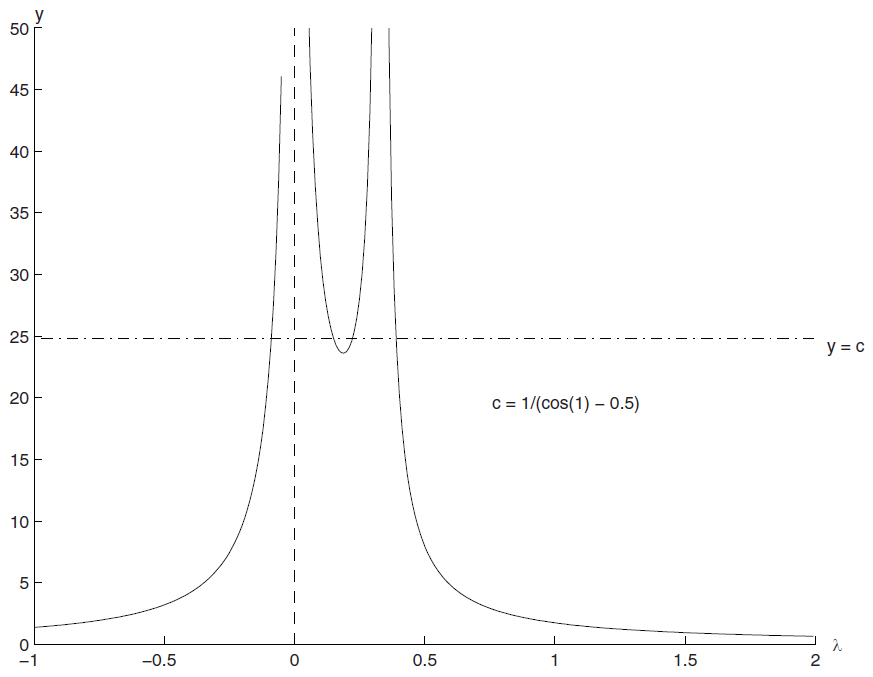
\includegraphics[width=\textwidth]{fig4.1}
	\caption{Gráfico de la parte izquierda de la desigualdad~\eqref{ej:3}}
	\label{fig:4.1}
\end{figure}

\endinput
%------------------------------------------------------------------------------------
% FIN DEL CAPÍTULO. 
%------------------------------------------------------------------------------------